\section{Marco Teórico}\label{sec:mt}

% =====================================================================
\subsection{Hidroponía y solución nutritiva}\label{sec:hidroponia}

\subsubsection{Producción hidropónica y sistemas de cultivo}\label{sec:sistemas}
La agricultura concentra alrededor del 70\,\% de las extracciones de agua del mundo, y la escasez de agua dulce limita la producción [21]. El cultivo sin suelo se plantea, en ese contexto, como una forma de producir en suelos no cultivables y de ahorrar agua, sobre todo en los sistemas cerrados, que recogen el drenaje y reutilizan la solución [22]. En el Ecuador, el boletín de la encuesta agropecuaria nacional no incluye una categoría para el cultivo hidropónico [23], y la hidroponía del país se conoce por casos: la producción comercial de lechuga de la Sierra [4] y los huertos urbanos y periurbanos [17]. En la sede Guayaquil de la Universidad Politécnica Salesiana, varios trabajos de titulación recientes han automatizado prototipos hidropónicos: el riego de una granja vertical que avisa si el pH sale de rango, pero se corrige a mano [24]; un sistema vertical con recirculación [25]; la conductividad eléctrica con un controlador difuso [26]; el caudal de la solución con un PID [27]; la temperatura y el riego de un invernadero de forraje [28], y el pH y la conductividad con dos lazos de histéresis [12].

Los sistemas de cultivo se distinguen por el medio en que crece la raíz (figura~\ref{fig:cultivo}a): el suelo, un sustrato orgánico o inorgánico, o directamente el agua [22]. Los métodos de riego principales son por superficie, por aspersión y el microrriego [21] (figura~\ref{fig:cultivo}b). Cuando el agua lleva disueltos los fertilizantes se habla de fertirriego, y con el mismo inyector se puede añadir ácido para llevar la alcalinidad del agua a un rango objetivo [29]: corregir el pH forma parte, desde el principio, del manejo del riego.

\figura{fig:cultivo}{fig01.pdf}{Sistemas de cultivo y métodos de riego}{Sistemas de cultivo y métodos de riego. (a) Clasificación de los sistemas de cultivo según el medio en que crece la raíz; la hidroponía, resaltada, es el caso de este trabajo. (b) Métodos de riego principales; cualquiera de ellos puede llevar los fertilizantes disueltos en el agua, como fertirriego. Elaborado por los autores (A. Morocho y K. Toledo, TikZ, 2026), a partir de [21, 22].}

La hidroponía es el cultivo de plantas sin suelo, en el que los nutrientes minerales llegan a la raíz disueltos en agua, de modo que la nutrición queda por entero en manos de la formulación [1, págs. 1–11]. Los sistemas hidropónicos se distinguen por cómo llega la solución a la raíz (figura~\ref{fig:sistemas}): en la película nutritiva (NFT), una lámina delgada recorre canales inclinados; en la raíz flotante, las plantas flotan sobre un depósito de solución aireada, y en el cultivo en sustrato, la solución se aplica por goteo. Las figuras~\ref{fig:nft} y~\ref{fig:flotante} muestran los dos primeros en invernadero. Se distinguen también por el destino del drenaje: en los sistemas abiertos se desecha, y en los cerrados, o recirculantes, vuelve al depósito y se reutiliza [1, págs. 1–11].

\figura{fig:sistemas}{fig02.pdf}{Sistemas hidropónicos según cómo llega la solución a la raíz}{Sistemas hidropónicos según cómo llega la solución a la raíz, en su variante recirculante: (a) película nutritiva (NFT), (b) raíz flotante y (c) cultivo en sustrato. En los tres, el depósito es el punto donde se mide y se corrige el pH. Elaborado por los autores (A. Morocho y K. Toledo, TikZ, 2026).}

Los sistemas recirculantes ahorran agua y fertilizante, pero su solución cambia de composición y de pH a medida que la raíz la recorre. Además, el cultivo sin suelo apenas amortigua esos cambios: un error de fertilización tiene consecuencias directas [22], y en la película nutritiva una interrupción del suministro afecta pronto al rendimiento [30]. El depósito es el punto natural de control: allí se mide, se corrige y se repone. Es también el escenario de este trabajo, en el que el depósito se reproduce como banco de ensayos sin cultivo.

\begin{figure}[H]\centering
\foto{fig:nft}{fig03.pdf}{Cultivo en película nutritiva (NFT)}{Cultivo de lechuga en película nutritiva (NFT), en invernadero. Foto de Izhamwong, Wikimedia Commons, CC~BY~3.0.}\hspace{10mm}
\foto{fig:flotante}{fig04.pdf}{Cultivo en raíz flotante}{Cultivo en raíz flotante, en invernadero. Foto de ArcadiYay, Wikimedia Commons, CC~BY-SA~4.0.}
\end{figure}

\subsubsection{Solución nutritiva y rango de pH}\label{sec:solucion}
La planta toma de la solución los macronutrientes y los micronutrientes en proporciones que la formulación fija de antemano [1, págs. 13–33], [2]. La concentración total se vigila con la conductividad eléctrica (CE) [1, págs. 35–87]. La CE y el pH se regulan por separado: la CE informa de cuánto nutriente hay, y el pH, de en qué forma química está. La solución se prepara a partir de concentrados que se mantienen separados (A, B y C), porque el calcio de uno y los fosfatos y sulfatos de otro precipitan si se juntan concentrados [1, págs. 35–87]. La formulación de este trabajo contiene unos 1,3\,mM de fosfato, aportados como KH$_2$PO$_4$, que junto con el carbonato del agua fijan su capacidad para resistir cambios de pH. Cuando la raíz crece en un sustrato, este aporta además su propio pH: la turba puede ser muy ácida, y la fibra de coco tiene un pH de entre 5 y 7 [22]. El banco de este trabajo no tiene cultivo ni sustrato.

El pH determina si la raíz puede absorber los nutrientes. Por encima del rango recomendado el hierro, el manganeso y el fósforo precipitan o forman especies poco disponibles; por debajo, la absorción de algunos cationes se reduce y otros elementos alcanzan concentraciones fitotóxicas [1, págs. 35–87], [2]. Incluso variaciones pequeñas tienen efecto medible en lechuga [3]. Por eso la práctica hidropónica mantiene el pH entre 5,5 y 6,5, con un valor deseado, o consigna, en torno a 6,0. En este trabajo, ese rango es el requisito del que se deriva todo lo demás: la incertidumbre admisible de la medición, el ancho de la zona muerta y el mayor cambio de pH admisible por dosis.

El pH de una solución nutritiva no permanece constante. Lo modifican cinco factores:
\begin{enumerate}
\item La absorción radicular, el factor dominante en un cultivo. Cuando la planta absorbe nitrato libera hidroxilo o bicarbonato y el pH sube; cuando absorbe amonio, baja [2, 31]. Por eso la perturbación típica de un cultivo hidropónico eleva el pH y la corrige la vía de ácido.
\item La alcalinidad del agua de preparación, su capacidad para neutralizar ácido, que en las aguas naturales se debe casi por completo al bicarbonato y al carbonato [32, págs. 163–172]:
\begin{equation}
\mathrm{ANC}=[\mathrm{HCO_3^-}]+2\,[\mathrm{CO_3^{2-}}]+[\mathrm{OH^-}]-[\mathrm{H^+}]\label{eq:anc}
\end{equation}
Se expresa en miligramos por litro de CaCO$_3$ equivalente (50\,mg/L corresponden a 1\,meq/L). El bicarbonato tampona la solución cerca del rango de trabajo, y por eso en el fertirriego se neutraliza antes de preparar la solución [15, 29]. La alcalinidad de diseño de este trabajo es de 80\,mg/L de CaCO$_3$ (1,6\,meq/L).
\item El intercambio de dióxido de carbono con la atmósfera (apartado~\ref{sec:equilibrio}).
\item La propia composición: el fosfato añadido aumenta la capacidad tampón, hasta el punto de que esta se ha propuesto como medida indirecta de la concentración de fosfato [33].
\item La temperatura, que reduce el oxígeno disuelto (de unos 9,1\,mg/L a 20\,°C a unos 8,3\,mg/L a 25\,°C) [32, págs. 212–216], desplaza los equilibrios ácido-base (apartado~\ref{sec:tampon}) y cambia la respuesta del electrodo (apartado~\ref{sec:temperatura}).
\end{enumerate}

% =====================================================================
\subsection{Fundamentos fisicoquímicos del pH}\label{sec:quimica}

\subsubsection{Equilibrio ácido-base de la solución}\label{sec:equilibrio}
El pH es el cologaritmo de la actividad del ion hidrógeno, $\mathrm{pH}=-\log_{10}a_{\mathrm{H^+}}$. Como la actividad de un ion individual no puede medirse, la IUPAC lo define de forma operacional, a partir de la tensión de una celda calibrada contra disoluciones patrón [34]: todo valor de pH depende de los patrones y del estado del electrodo. A 25\,°C, $K_w=10^{-14{,}00}$ y la neutralidad corresponde a pH 7,00; el rango hidropónico es moderadamente ácido.

Un tampón es un par ácido-base conjugado que resiste los cambios de pH; su efecto es máximo cuando el pH coincide con el p$K_a$ del par y se extiende más o menos una unidad a cada lado. En la solución nutritiva actúan dos: el fosfato de la formulación y el carbonato, que viene de la alcalinidad del agua y del CO$_2$ disuelto. A 25\,°C y fuerza iónica nula, sus constantes son p$K_a$ = 2,148; 7,198 y 12,375 para el fosfato, y p$K'_a$ = 6,352 y 10,329 para el carbonato [32, págs. 92–97, 150–157]. El primer p$K'_a$ del carbonato cae dentro del rango objetivo, y el segundo del fosfato, justo por encima del rango de caracterización, de 5,0 a 7,0 (figura~\ref{fig:especies}).

\figura{fig:especies}{fig05.pdf}{Fracción de cada especie del fosfato y del carbonato frente al pH}{Fracción de cada especie frente al pH, calculada con las constantes a 25\,°C y fuerza iónica nula, con el rango objetivo sombreado. (a) Fosfato: en el rango objetivo predomina H$_2$PO$_4^-$, y su segundo p$K_a$, 7,20, queda justo por encima. (b) Carbonato: su primer p$K'_a$, 6,35, cae dentro del rango objetivo. Elaborado por los autores (A. Morocho y K. Toledo, MATLAB, 2026).}

El modelo del proceso describe el depósito con cuatro cantidades que se conservan cuando ácidos y bases reaccionan: el fosfato total $n_P$, el carbono inorgánico total $n_C$, los iones fuertes netos $n_S$ y el volumen $V_T$ [35]. Cada dosis se suma a esas cantidades, y la no linealidad queda en el paso de la composición al pH, que es la condición de electroneutralidad. Con $h=[\mathrm{H^+}]$, $S=n_S/V_T$, $C_P=n_P/V_T$ y $C_C=n_C/V_T$:
\begin{equation}
h-\frac{K_w}{h}+S-C_P\,\bar z_P(h)-C_C\,\bar z_C(h)=0\label{eq:electro}
\end{equation}
donde $\bar z_P$ y $\bar z_C$ son las cargas negativas medias por átomo de fósforo y de carbono [32, págs. 127–130]. De esta ecuación sale la curva de titulación del modelo.

En el banco, la descarga de la recirculación cae sobre la superficie del depósito, y el CO$_2$ escapa hasta equilibrarse con la atmósfera, según la ley de Henry [32, págs. 157–163, 212–216]. Por eso cada lote se desgasifica antes de ensayar (pre-despojo, apartado~\ref{sec:hid}). Después, el carbono inorgánico lo fija el aire, la ganancia del lazo ya no depende de la dureza del agua y el tampón dominante es el fosfato de la formulación.

\subsubsection{Reactivos, capacidad tampón y curva de titulación}\label{sec:tampon}
Este trabajo baja el pH con ácido sulfúrico y lo sube con hidróxido de potasio. Los dos son electrolitos fuertes entre pH 5 y 7: modifican solo los iones fuertes netos y no añaden capacidad tampón, como haría un reactivo débil [32, págs. 92–97], así que la curva de titulación no se desplaza mientras se dosifica. El sulfato y el potasio, además, ya forman parte de la solución nutritiva. Los dos reactivos se adquieren valorados a la misma normalidad, de modo que las dos bombas producen idealmente el mismo cambio a un mismo pH.

La capacidad tampón se mide con el valor tampón de Van Slyke [36], los equivalentes de ácido o de base fuerte por litro que desplazan el pH una unidad:
\begin{equation}
\beta(\mathrm{pH})\equiv\left|\frac{dS}{d\,\mathrm{pH}}\right|\label{eq:beta}
\end{equation}
La curva de titulación representa el pH frente a la cantidad de reactivo añadida, y su pendiente es la inversa de $\beta$, salvo el factor de volumen. La ganancia local del proceso, el cambio de pH por cada mililitro de reactivo, sale del balance de cargas:
\begin{equation}
K_p=\left|\frac{d\,\mathrm{pH}}{dV}\right|=\frac{c_{\text{ef}}}{V_T\,\beta(\mathrm{pH})}\label{eq:kp}
\end{equation}
donde $c_{\text{ef}}$ es la concentración del reactivo en equivalentes por litro y $V_T$ el volumen del depósito (con $V$ en mililitros, la expresión lleva el factor $10^{-3}$). Como $\beta$ cambia con el pH, la ganancia también: según el modelo del banco, unas 15 veces entre pH 5,0 y 7,0 (tabla~\ref{tab:beta}). Una sintonía de ganancia fija no puede ser adecuada en todo el rango [14, págs. 53–59], y el controlador de este trabajo calcula la dosis con la curva de titulación (apartado~\ref{sec:planta}). La ecuación~\eqref{eq:kp} indica también cómo reducir la ganancia: el volumen es un dato de la instalación, pero al diluir el reactivo cada dosis mínima mueve menos el pH.

Las constantes de equilibrio cambian con la temperatura [32, págs. 52–57], y con ellas el pH de una solución de composición fija. El orden de magnitud lo dan los patrones de calibración (tabla~\ref{tab:patrones}): el de 6,86, un tampón de fosfato como el que domina la solución, varía unas 0,004 unidades de pH por grado. En la ventana de $22\pm3$\,°C, eso supone del orden de $\pm0{,}01$\,pH, diez veces menos que la incertidumbre de la medición. Este cambio es químico, y el instrumento no debe corregirlo.

% =====================================================================
\subsection{Medición del pH y compensación por temperatura}\label{sec:medicion}

\subsubsection{Electrodo de pH y sondas digitales}\label{sec:electrodo}
El pH se mide con un electrodo de vidrio, cuya membrana desarrolla una diferencia de potencial que depende de la actividad del ion hidrógeno, frente a un electrodo de referencia. La tensión de la celda sigue idealmente la ecuación de Nernst:
\begin{equation}
E=E_0-\frac{2{,}303\,R\,T}{F}\,\mathrm{pH}\label{eq:nernst}
\end{equation}
donde $R$ es la constante de los gases, $F$ la de Faraday y $T$ la temperatura absoluta. A 25\,°C la pendiente teórica es de $-59{,}16$\,mV por unidad de pH [37, págs. 69–71]. En un electrodo combinado, el de vidrio y el de referencia (plata y cloruro de plata en cloruro de potasio) van en el mismo cuerpo, y el circuito se cierra a través de una unión líquida, un diafragma poroso [37, págs. 72–76, 91–101] (figura~\ref{fig:electrodo}). La pendiente real es menor que la teórica y baja con el uso, el potencial a pH neutro deriva con el tiempo [37, págs. 102–106], y la unión líquida puede obstruirse con precipitados de la muestra [14, págs. 92–102]. En una solución con calcio y fosfato las dos cosas son esperables, y el electrodo se calibra periódicamente contra patrones.

\figura{fig:electrodo}{fig06.pdf}{Esquema de un electrodo combinado de pH}{Esquema de un electrodo combinado de pH. El electrodo de vidrio, con su solución interna y su electrodo interno, mide frente al de referencia, que cierra el circuito a través del diafragma. En una sonda digital como la de este trabajo, el cabezal integra además el acondicionamiento, la conversión analógico-digital, la compensación de temperatura y la comunicación Modbus RTU. No está a escala. Elaborado por los autores (A. Morocho y K. Toledo, TikZ, 2026).}

En un sensor analógico, el electrodo se cablea hasta un acondicionador de muy alta impedancia y un convertidor analógico-digital, y cada eslabón añade incertidumbre. Una sonda digital integra todo eso y entrega el pH ya calculado por un bus. La de este trabajo (figura~\ref{fig:sonda}) se comunica por Modbus RTU sobre RS-485, declara una exactitud de $\pm0{,}1$\,pH y una resolución de 0,01\,pH en un rango de 0 a 14, compensa la temperatura internamente y se alimenta de 12 a 24\,V [57]. Con ella, la cuantización y el ruido del cable quedan dentro de la exactitud declarada, y una interferencia produce una trama corrupta o perdida, más fácil de detectar que una lectura ruidosa. La desventaja es que no expone la tensión del electrodo: su pendiente no puede medirse desde fuera, y su estado se comprueba con el error en un punto de verificación independiente.

\subsubsection{Incertidumbre de medida y calibración}\label{sec:incertidumbre}
Los términos son los del Vocabulario Internacional de Metrología [38]. El error de medida es la diferencia entre el valor medido y un valor de referencia. La resolución es la menor variación que produce un cambio perceptible de la indicación. La repetibilidad es la concordancia entre mediciones repetidas en las mismas condiciones y en un intervalo corto, y la deriva, la variación continua de la indicación con el tiempo. La Guía para la Expresión de la Incertidumbre de Medida (GUM) establece cómo se combinan las contribuciones [39]. Las de tipo A se evalúan con estadística sobre observaciones repetidas ($u=s/\sqrt{n}$ para la media de $n$ lecturas); las de tipo B, con información previa, como las especificaciones del fabricante ($u=a/\sqrt{3}$ para un semiancho $a$ con distribución rectangular). Para un mensurando $y=f(x_1,\dots,x_N)$ con entradas no correlacionadas,
\begin{equation}
u_c^2(y)=\sum_{i=1}^{N}\left(\frac{\partial f}{\partial x_i}\right)^{2}u^2(x_i)\label{eq:gum}
\end{equation}
y la incertidumbre expandida es $U=k\,u_c$, con $k=2$ para un nivel de confianza de alrededor del 95\,\% [39].

\tabla{tab:presupuesto-u}{tab01.pdf}{Presupuesto de incertidumbre estimado a priori a partir de las especificaciones}

La tabla~\ref{tab:presupuesto-u} aplica la ecuación~\eqref{eq:gum} a las especificaciones publicadas; es una estimación \emph{a priori}, que sirve para dimensionar el diseño, y el presupuesto real se construye con datos medidos (apartado~\ref{sec:carmed}). El electrodo aporta casi el 96\,\% de la varianza. En este trabajo, $U$ es el margen de error de la medición del que hablan el Problema y los objetivos: contra él se contrasta cada indicador de desempeño, y de él salen el mayor cambio de pH admisible por dosis y el ancho de la zona muerta. El riesgo es que casi toda la estimación descansa en la exactitud que declara el fabricante de una sonda de bajo costo, y la incertidumbre medida podría superar el criterio $U\le0{,}15$\,pH. Si ocurre, el diseño no se invalida: la zona muerta de 0,25\,pH sigue siendo admisible mientras $U\le0{,}25$\,pH (ecuación~\eqref{eq:banda}), la dilución se vuelve a comprobar con la ecuación~\eqref{eq:regla} y el valor medido se declara con los resultados.

La calibración de dos puntos fija el cero y la pendiente con dos patrones que encierran el rango de trabajo; un tercero, que no entra en la calibración, la verifica. La sonda de este trabajo calibra contra la serie china GB (4,00; 6,86 y 9,18) y no contra la serie NIST [57]: calibrar con 7,00 donde espera 6,86 introduciría un sesgo de 0,14\,pH. Aquí se calibra con 6,86 como cero y 4,00 como pendiente, y el 9,18 se reserva para la verificación. Sin certificado del lote de los patrones no puede reclamarse trazabilidad a las unidades del SI, aunque el patrón pesa poco en la incertidumbre.

\subsubsection{Efecto de la temperatura y su compensación}\label{sec:temperatura}
Además del efecto químico (apartado~\ref{sec:tampon}), la temperatura cambia la respuesta del electrodo: su pendiente es proporcional a la temperatura absoluta (ecuación~\eqref{eq:nernst}), y una misma tensión corresponde a un pH distinto según la temperatura de la muestra. El error es nulo en el punto isopotencial, cerca de pH 7 en los electrodos comerciales, y crece al alejarse de él (figura~\ref{fig:temp}a). La compensación automática mide la temperatura y ajusta la pendiente; si la temperatura que usa es errónea, queda un error
\begin{equation}
\varepsilon_{\mathrm{pH}}\approx\frac{\Delta T}{T}\,\bigl|\mathrm{pH}-\mathrm{pH}_{\text{iso}}\bigr|\label{eq:comp}
\end{equation}
Con un error de 0,5\,°C, en pH 5,5 son unos 0,0025\,pH (figura~\ref{fig:temp}b), despreciables frente a la exactitud del electrodo. En este trabajo la temperatura no se regula: se mide para que la lectura sea correcta y para registrar en qué condiciones se ensayó.

\figura{fig:temp}{fig08.pdf}{Efecto de la temperatura en la medición del pH}{Efecto de la temperatura en la medición del pH. (a) Tensión de un electrodo ideal frente al pH a 10, 25 y 40\,°C, según la ecuación~\eqref{eq:nernst}: la pendiente crece con la temperatura absoluta, y las tres rectas se cruzan en el punto isopotencial, en pH 7. (b) Error de pH que produce un error de 0,5 o de 3\,°C en la temperatura de la compensación, según la ecuación~\eqref{eq:comp}, a 22\,°C, frente a la incertidumbre $U$. El rango objetivo va sombreado. Elaborado por los autores (A. Morocho y K. Toledo, MATLAB, 2026).}

La compensación de la sonda tiene tres limitaciones: corrige solo la pendiente, supone que su sensor está a la temperatura de la membrana y el fabricante no documenta el algoritmo [57]. Las dos primeras se mantienen pequeñas ensayando dentro de una ventana estrecha y con variaciones lentas. La tercera se aborda desde fuera, con una sonda de temperatura independiente: un sensor digital DS18B20 en vaina de acero inoxidable (figura~\ref{fig:ds18b20}), con una exactitud de $\pm0{,}5$\,°C entre $-10$ y $+85$\,°C, bus 1-Wire y una resolución de 0,0625\,°C a 12 bits [58]. La compensación se verifica de dos maneras, sin ensayos adicionales: comparando la temperatura interna que la sonda de pH entrega por Modbus con la del DS18B20, y leyendo el patrón de 9,18, cuyo valor nominal depende de la temperatura (tabla~\ref{tab:patrones}): a 22\,°C vale 9,21, y contrastarlo con el nominal atribuiría a la sonda un error de 0,03\,pH que procede del patrón.

\begin{figure}[H]\centering
\foto{fig:sonda}{fig07.pdf}{Sonda digital de pH Veinasa-PH06}{Sonda digital de pH Veinasa-PH06. Imagen del manual del fabricante [57].}\hspace{10mm}
\foto{fig:ds18b20}{fig09.pdf}{Sonda de temperatura DS18B20}{Sonda de temperatura DS18B20 en vaina de acero inoxidable, DFRobot DFR0198 [58].}
\end{figure}

\tabla{tab:patrones}{tab02.pdf}{Valor nominal de los patrones de la serie GB y del patrón 7,00 frente a la temperatura, según el manual de la sonda}

% =====================================================================
\subsection{Dosificación de soluciones ácidas y básicas}\label{sec:dosificacion}

\subsubsection{Bomba peristáltica y dosis por revoluciones}\label{sec:bomba}
Dosificar es entregar una cantidad conocida de un líquido. La cantidad puede fijarse por volumen, con una bomba de desplazamiento positivo; por tiempo, con una bomba de caudal supuesto, o por masa, que es el método de referencia en laboratorio. En un lazo de control importan la repetibilidad de la dosis y la menor dosis que puede entregarse, porque fijan la resolución con que el actuador mueve el pH [14, págs. 178–181]; un error sistemático del volumen lo absorbe la realimentación.

Una bomba peristáltica desplaza el líquido por la oclusión sucesiva de un tubo flexible, que aprietan los rodillos de un rotor (figura~\ref{fig:peristaltica}). El líquido solo toca el interior del tubo [13], que en la bomba elegida es de BPT [59] y cuya compatibilidad con los reactivos se comprueba en la tabla de su fabricante [60]. El tubo es un consumible: se fatiga y su desplazamiento cambia. La bomba es una Kamoer KPAS-100 (figura~\ref{fig:kamoer}), de tres rodillos y tubo de 3,2\,mm de diámetro interior, que declara 110\,mL/min a 350\,rpm [59]:
\begin{equation}
V_{\text{rev}}=\frac{110\ \text{mL/min}}{350\ \text{rpm}}=0{,}314\ \text{mL por revolución}\label{eq:vrev}
\end{equation}
Mantener la exactitud es más difícil cuanto menor es el volumen: en un conjunto de datos de dosificación peristáltica, el coeficiente de variación pasa del 0,28\,\% con 2,0\,mL al 1,43\,\% con 0,2\,mL [13].

\figura{fig:peristaltica}{fig10.pdf}{Principio de la bomba peristáltica}{Principio de la bomba peristáltica. Los rodillos del rotor cierran el tubo contra la carcasa y encierran entre dos oclusiones un volumen que empujan hacia la salida; con tres rodillos, cada revolución entrega tres de esos volúmenes. Cifras nominales de la bomba de este trabajo; no está a escala. Elaborado por los autores (A. Morocho y K. Toledo, TikZ, 2026).}

La bomba usa un motor paso a paso de 200 pasos por revolución, que el controlador subdivide en micropasos (1600 por revolución con 1/8) [61]. La dosis se pide como un número de pasos y no depende del tiempo de encendido. Pero la resolución angular del motor no es la de la dosis: un paso de rodillo, de 0,105\,mL, no corresponde a un número entero de pasos, y una dosis parcial deja el tubo en otra fase de oclusión. La unidad de dosificación de este trabajo es por eso la revolución completa. El motor se controla en lazo abierto, sin sensor de posición [50]: sigue los pasos mientras el par de la carga, que aquí impone la oclusión del tubo, no supere su par máximo a esa velocidad; si lo supera, pierde pasos sin que el controlador lo detecte. Por eso la corriente de los bobinados solo se sube si la bomba pierde pasos, y el volumen entregado no se deduce de los pasos: se mide por gravimetría.

\begin{figure}[H]\centering
\foto{fig:kamoer}{fig11.pdf}{Bomba peristáltica Kamoer KPAS-100}{Bomba peristáltica Kamoer KPAS-100 con su motor paso a paso. Imagen generada por computadora, del fabricante [59].}
\end{figure}

\subsubsection{Dosis mínima, mezcla y sobredosificación}\label{sec:dosismin}
La dosis mínima repetible, $\Vmin$, que es la menor dosis confiable de los objetivos, es el menor número entero de revoluciones cuya dosis mantiene un coeficiente de variación no superior al 5\,\%. Es un resultado experimental, que se espera del orden de una revolución y se determina pesando las dosis. Con ella se formula la regla de dimensionamiento, que relaciona el actuador, el proceso y el instrumento: el cambio de pH que produce la dosis mínima repetible no debe superar, en ningún punto del rango objetivo, la mitad de la incertidumbre expandida de la medición:
\begin{equation}
\Vmin\cdot\left|\frac{d\,\mathrm{pH}}{dV}\right|\le\frac{U}{2}\label{eq:regla}
\end{equation}
Así la resolución del actuador queda por debajo de lo que la sonda distingue. La regla es una propuesta propia de este trabajo, cuyos argumentos se dan en el apartado~\ref{sec:arq}. Se cumple diluyendo el reactivo, una técnica documentada para ampliar el rango útil de la dosificación [14, págs. 194–196], con un límite: el reactivo añadido aumenta el volumen del depósito y diluye la solución (apartado~\ref{sec:carbom}).

El reactivo no llega al electrodo en el instante en que se dosifica: gotea en el chorro de retorno de la recirculación, y el electrodo sigue la composición del depósito con un retardo de transporte y una mezcla de primer orden. Si el depósito se comporta como un tanque perfectamente mezclado, su constante de mezcla es $\tau_{\text{mez}}\approx V_T/Q_{\text{recirc}}$: con 10\,L y unos 400\,L/h, unos 90\,s. Más caudal mezclaría antes, pero la bomba de recirculación cedería más calor a la solución; por eso su caudal se ajusta reduciendo su tensión.

La sobredosificación tiene dos orígenes. El controlador puede pedir de más, lo que se previene con la ley de control y la capa de seguridad. O el actuador puede entregar lo que no se le pidió: una bomba peristáltica detenida no es una válvula, y el tubo puede actuar como sifón (apartado~\ref{sec:hid}). El fallo opuesto es la dosis sin efecto, por un tubo roto, un depósito vacío o un electrodo muerto; detectarlo no es inmediato, porque en la región tamponada una dosis correcta mueve muy poco el pH (apartado~\ref{sec:seg}).

% =====================================================================
\subsection{Control automático del pH}\label{sec:teocontrol}

\subsubsection{Métodos de control y lazo cerrado}\label{sec:metodos}
El pH de la solución se corrige añadiendo un ácido cuando sube y una base cuando baja. Los métodos se diferencian en quién decide la corrección y con qué información (tabla~\ref{tab:metodos}). En los prototipos académicos revisados en el Problema, la dosis se decide con lazos de histéresis o PID [10, 12], con reglas difusas [5, 6, 11, 16] o con una dosis recomendada por litro [8], y una revisión de 89 estudios encontró que predominan el lazo de realimentación convencional y la lógica difusa [40]. El método de este trabajo es un control por rango dividido con zona muerta que calcula cada dosis con la curva de titulación. Linealizar el control del pH con esa curva es una técnica conocida en los procesos de neutralización [14, págs. 212–216], [35, 42].

\tabla{tab:metodos}{tab03.pdf}{Métodos de control del pH en la producción agrícola}

Un sistema de control en lazo cerrado compara la variable controlada, que mide un sensor, con su consigna, y actúa sobre el proceso según el error [18, secs. 1.1 y 1.5]. La realimentación corrige las perturbaciones sin medirlas: basta con que su efecto aparezca en la medición. El controlador de este trabajo es digital y decide a intervalos discretos [18, sec. 11.5]: repite cuatro fases, medir, decidir, dosificar y esperar el asentamiento (figura~\ref{fig:lazo}). Como al decidir la planta está prácticamente asentada, el controlador no ve dinámica: ve una relación fija entre la dosis acumulada y el pH, cuya ganancia cambia con el pH.

\figura{fig:lazo}{fig12.pdf}{Diagrama de bloques del lazo de control del pH}{Diagrama de bloques del lazo de control del pH por rango dividido con actuación discreta. El recinto discontinuo delimita lo que se ejecuta en el microcontrolador; la linealización aparece dos veces porque la inversa de la curva de titulación se aplica tanto a la consigna como a la medida. En rojo, el balance de cargas, que es la relación no lineal entre la composición y el pH, situado entre la dinámica de mezcla y la del electrodo. Elaborado por los autores (A. Morocho y K. Toledo, TikZ, 2026).}

\subsubsection{Dinámica del proceso de neutralización}\label{sec:dinamica}
El control de pH reúne tres dificultades [14, págs. 1–9]: la no linealidad (la ganancia varía unas 15 veces en el rango de trabajo), el retardo y, en este trabajo, un actuador formado por dos bombas que solo añaden reactivo, cada una en una dirección y en dosis cuantizadas. El proceso encadena la mezcla y el transporte, que actúan sobre la composición; el balance de cargas, que la convierte en pH sin dinámica propia, y la respuesta del electrodo. Que la no linealidad quede entre dos dinámicas lineales es lo que orienta el diseño del control [35, 42]. Como el fabricante no especifica la constante de tiempo del electrodo [57], se identifica la dinámica del conjunto tanque-electrodo, reducida a un primer orden con retardo:
\begin{equation}
G(s)=\frac{K_p\,e^{-\theta s}}{\tau s+1}\label{eq:fopdt}
\end{equation}
Es una aproximación local: su ganancia es la pendiente de la curva de titulación en el punto donde se identifica. Lo que aporta son el retardo $\theta$ y la constante de tiempo $\tau$, que se identifican sobre la respuesta a las propias dosis de la titulación (apartado~\ref{sec:planta}), con el método de dos puntos (28,3 y 63,2\,\% del valor final) refinado por mínimos cuadrados. Un modelo identificado debe validarse con datos distintos de los del ajuste, y sus residuos no deben presentar estructura [43]. La bondad del ajuste se mide con
\begin{equation}
\mathrm{FIT}=\left(1-\frac{\lVert y-\hat y\rVert}{\lVert y-\bar y\rVert}\right)\times100\ \%\label{eq:fit}
\end{equation}
donde $y$ es la respuesta medida, $\hat y$ la simulada y $\bar y$ la media de $y$. La espera entre dosis se fija en $T_s=\theta+3\tau$, y en la titulación, donde se busca el valor asentado, en $\theta+5\tau$.

\subsubsection{Zona muerta y rango dividido}\label{sec:zonamuerta}
En el control de todo o nada, el actuador se enciende cuando la variable cruza un umbral; para que el ruido no lo haga conmutar sin parar se separan los umbrales de encendido y apagado (histéresis) [18, sec. 1.6]. Cuando a la variable se le exige un rango de tolerancia, el controlador puede dejar de actuar dentro de un rango más estrecho, la zona muerta. Si dos actuadores de efecto opuesto actúan sobre la misma variable, la salida se reparte entre ellos con un control por rango dividido (\emph{split-range}): el signo del error decide qué bomba actúa [14, págs. 184–186]. La tabla~\ref{tab:logica} resume la lógica, con una zona muerta de semiancho $\delta$ centrada en la consigna: fuera de ella se actúa sobre el error completo.

\tabla{tab:logica}{tab04.pdf}{Lógica del control por rango dividido con zona muerta}

La zona muerta impide que las dos bombas se corrijan una a otra alrededor de la consigna, reduce el número de dosis y evita reaccionar al ruido. También protege frente al ciclo límite, propio de los lazos con actuación cuantizada [18, sec. 1.6]: si la dosis mínima moviera el pH más que el ancho de la zona muerta, el lazo oscilaría entre las dos bombas consumiendo reactivo. La regla de la ecuación~\eqref{eq:regla} busca evitarlo, y el ancho se fija contra la incertidumbre de la medición, en $\delta=0{,}25$\,pH (apartado~\ref{sec:desempeno}).

\subsubsection{Control por demanda de reactivo y estabilidad}\label{sec:demanda}
Cada dosis se acumula en el depósito. Si el controlador calcula el volumen de la decisión $k$ como $u[k]=\gamma\,e[k]/\hat K_p$, con una estimación $\hat K_p$ de la ganancia, el error evoluciona como
\begin{equation}
e[k+1]=\left(1-\gamma\,\frac{K_p}{\hat K_p}\right)e[k]\label{eq:lazo}
\end{equation}
Con la ganancia bien estimada y $\gamma=1$ el error se anula en una decisión; si la ganancia real es menor hacen falta varias dosis, si es mayor cada dosis rebasa la consigna, y si es más del doble el lazo oscila sin converger. Un controlador de ganancia fija, sea proporcional, PI o PID, se sintoniza con una sola ganancia, normalmente la de la consigna, y pide de menos donde la ganancia real es menor y de más donde es mayor (figura~\ref{fig:leyes}). La comparación experimental con un PID queda fuera del alcance.

El control por demanda de reactivo deshace primero la no linealidad [35, 42]: trabaja en volumen de reactivo y no en unidades de pH. Lee de la curva de titulación inversa, $\mathcal V(\mathrm{pH})$, el volumen acumulado que corresponde al pH medido y a la consigna, y dosifica una fracción $\gamma$ de la diferencia:
\begin{equation}
V_{\text{cmd}}=\gamma\,\klote\,\bigl|\mathcal V(\pHm{consigna})-\mathcal V(\pHm{medido})\bigr|\label{eq:vcmd}
\end{equation}
El factor $\klote$ reescala la curva a cada lote y se obtiene en la autocalibración (apartado~\ref{sec:control}). El controlador aplica el 70\,\% de la demanda, $\gamma=0{,}70$, porque una dosis excesiva solo podría compensarse con el reactivo contrario; es la misma prudencia que se recomienda al ajustar el pH a mano [7]. No tiene acción integral, porque el depósito ya integra cada dosis, y el error final no es nulo: se contrasta con $U$. Otros trabajos abordan la misma no linealidad con control predictivo adaptativo [41]; usar la curva medida es más simple en un microcontrolador, donde se graba como una tabla. La idea no es nueva: lo que aporta este trabajo es llevarla a un prototipo que dosifica por lotes con una bomba de pasos discretos, y medir su desempeño frente a la incertidumbre de la medición.

En un lazo continuo, la estabilidad, el sobrepaso y el tiempo de estabilización se leen de la respuesta a un escalón [18, sec. 6.3]. En el lazo de dosificación discreta se deducen de la ecuación~\eqref{eq:lazo}: es estable si el factor $1-\gamma K_p/\hat K_p$ está entre $-1$ y 1, y hay sobrepaso si es negativo. Con $\gamma=0{,}70$, el error no cambia de signo mientras la ganancia real no supere 1,43 veces la estimada, y el lazo es estable hasta 2,86 veces. El tiempo de estabilización depende sobre todo del número de dosis, porque cada una va seguida de una espera $T_s$.

Una perturbación es toda entrada que modifica la variable controlada y que el controlador no manipula [18, sec. 2.3]; la principal es la absorción radicular, que eleva el pH de forma lenta y continua [2, 31]. La prealimentación exigiría medirla [18, sec. 1.2], lo que no es práctico, así que el control de pH hidropónico es casi siempre de realimentación. En un lazo por lotes, una perturbación lenta se corrige con dosis sucesivas cada vez que el pH sale de la zona muerta, y una sostenida que el controlador no logra compensar la detiene el límite de volumen acumulado. Para los ensayos, la perturbación se estandariza con un bolo de volumen fijo (apartado~\ref{sec:ensayos}).

% =====================================================================
\subsection{Sistema embebido y diseño mecánico}\label{sec:embebido}

\subsubsection{Microcontrolador, adquisición y comunicación}\label{sec:micro}
Un sistema embebido es un computador dedicado a una función dentro de un sistema mayor; cuando esa función es medir y modificar un proceso físico, el conjunto es un sistema ciberfísico, en el que el programa no puede separarse de la dinámica del proceso ni del tiempo [44, pág. 2]. Un microcontrolador reúne en un circuito el procesador y sus periféricos, que funcionan en paralelo y avisan con interrupciones [45, págs. 542.e3, 542.e39]. Frente al autómata programable, más caro y menos flexible para cálculos a medida, y al computador de placa única, cuyo sistema operativo no garantiza plazos, ofrece tiempos deterministas y bajo consumo. El firmware puede organizarse como un bucle principal o sobre un sistema operativo de tiempo real [19, págs. 1–18]; el primero es más simple y predecible con pocas tareas, y es el de este trabajo.

El controlador se implementa en una placa Nucleo-64 con el microcontrolador STM32G474RE (figura~\ref{fig:nucleo}), un Arm Cortex-M4 de hasta 170\,MHz con unidad de coma flotante, depurador ST-LINK con puerto serie virtual por USB [63, 64, 65] y un temporizador de vigilancia independiente, con oscilador propio [64]. La elección no es crítica: como el pH llega ya digitalizado, el microcontrolador no forma parte de la cadena de medición.

RS-485 es una capa física de comunicación serie diferencial, y sobre ella Modbus RTU define un protocolo maestro-esclavo: el microcontrolador envía una petición y la sonda responde. Cada trama lleva la dirección, un código de función, los datos y un código de redundancia cíclica (CRC) de 16 bits [46]. La sonda entrega el pH, su número de decimales y la temperatura interna con la función 3 [57], y la temperatura independiente se lee por 1-Wire, con una conversión de 750\,ms [58]. Cada lectura se valida: se rechaza si está fuera del rango físico o si la trama llega corrupta o tarde, y una trama perdida es ausencia de dato, no se sustituye por la anterior. La tasa de errores de trama, con la recirculación parada y en marcha, mide la integridad del enlace. Filtrar reduce el ruido a costa de retardo: promediar $n$ lecturas independientes divide su desviación típica por $\sqrt{n}$ [39], lo que se usa en la autocalibración del lote; en el lazo no se filtra, porque la espera ya deja la planta casi en reposo.

\begin{figure}[H]\centering
\foto{fig:nucleo}{fig13.pdf}{Placa Nucleo-G474RE}{Placa Nucleo-G474RE, con el microcontrolador STM32G474RE [66].}\hspace{10mm}
\foto{fig:tmc}{fig14.pdf}{Controlador de motor TMC2209}{Controlador de motor TMC2209 V1.3, de BIGTREETECH, con su disipador [67].}
\end{figure}

\subsubsection{Etapa de potencia, protecciones y supervisión}\label{sec:potencia}
Las salidas de un microcontrolador no pueden alimentar un motor, y entre los dos se pone una etapa de potencia. Cada bomba de reactivo se acciona con un controlador TMC2209 (figura~\ref{fig:tmc}), que alimenta las bobinas desde el riel de 24\,V, regula su corriente (de 4,75 a 29\,V y hasta 2\,A eficaces) y recibe dos señales: STEP, un pulso por micropaso, y DIR, el sentido de giro [61]. Su patilla de habilitación sirve de segundo nivel del enclavamiento que impide activar las dos bombas a la vez. La tabla~\ref{tab:riesgos} indica los riesgos eléctricos del banco y la protección de cada uno: el fusible abre el circuito ante una sobrecorriente; el interruptor diferencial, cuando parte de la corriente vuelve por otro camino [47]; el diodo de descarga extingue el pico de tensión de una carga inductiva [45, págs. 542.e55–542.e56], y el aislamiento divide el circuito en dominios con fuentes separadas [47].

\tabla{tab:riesgos}{tab05.pdf}{Riesgos eléctricos del prototipo y protección que responde a cada uno}

En un sistema de tiempo real, un resultado correcto que llega tarde es un fallo [19, págs. 1–18]. Aquí conviven escalas muy distintas: el periodo de decisión es de unos cinco minutos, y los pasos de los motores y las tramas Modbus exigen una puntualidad del orden del milisegundo, que se deja a los temporizadores y a los periféricos. El secuenciador se implementa como una máquina de estados finitos (figura~\ref{fig:estados}), con la que queda explícito lo que hay que verificar: que desde ningún estado se puedan activar las dos bombas, que un fallo detectado lleve al estado de fallo y que un bloqueo del firmware termine en un reinicio con las bombas detenidas.

\subsubsection{Materiales y estructura del banco}\label{sec:materiales}
En el banco los depósitos son recipientes comerciales, y lo que se diseña es el bastidor que los sostiene, con los soportes de la sonda y de las puntas de goteo. Sus requisitos son cinco: la carga, del orden de 20\,kg; la rigidez, para que no cambien las alturas de las que depende el funcionamiento; la resistencia química de las partes que pueden mojarse; la contención de un derrame, separada de la electrónica, y el acceso para mantenimiento. La compatibilidad química se comprueba en las tablas de los fabricantes, que son una guía basada en ensayos breves de inmersión [68]. Los dos reactivos quedan por debajo del 10\,\% en masa, y la tabla~\ref{tab:compat} recoge los materiales candidatos: los dos plásticos resisten los dos reactivos, y entre los metales solo el acero inoxidable 316 recibe una calificación que no lo descarta.

\tabla{tab:compat}{tab06.pdf}{Compatibilidad química de los materiales candidatos con los reactivos del banco, según las tablas de los fabricantes}

El método de Ashby ordena la elección de un material en cuatro pasos [48, cap. 4], [49]: la traducción de los requisitos en función, restricciones, objetivo y variables libres; el filtrado de los materiales que no cumplen las restricciones; la ordenación de los que quedan con un índice de material, y la documentación de los pocos candidatos finales. Para una viga de longitud $L$ y sección cuadrada cuya rigidez a flexión no debe bajar de $S^{*}$, la masa resulta
\begin{equation}
m=\left(\frac{12\,S^{*}}{C}\right)^{1/2}L^{5/2}\,\frac{\rho}{E^{1/2}}\label{eq:ashby}
\end{equation}
con $E$ el módulo de Young, $\rho$ la densidad y $C$ una constante de los apoyos y la carga: a igual rigidez, la viga más ligera es la del material con mayor índice $M=E^{1/2}/\rho$, o $E^{1/2}/(C_m\,\rho)$ si el objetivo es el costo, con $C_m$ el precio por kilogramo [49]. Su aplicación al bastidor lleva a elegir el tubo de PVC rígido de presión (figura~\ref{fig:pvc} y apartado~\ref{sec:hid}).

\begin{figure}[H]\centering
\foto{fig:pvc}{fig15.pdf}{Tubería de PVC roscable}{Tubería de PVC roscable para agua fría, de Plastigama Wavin [71].}
\end{figure}

% =====================================================================
\subsection{Validación experimental de sistemas de medición y control}\label{sec:validacion}

\subsubsection{Instrumentos de referencia y error de medición}\label{sec:referencias}
La verificación aporta evidencia objetiva de que un elemento cumple requisitos especificados, y la validación es una verificación en la que esos requisitos son los adecuados para un uso previsto [38]. Toda verificación descansa en instrumentos de referencia, y la trazabilidad metrológica exige una cadena ininterrumpida y documentada de calibraciones [38]. Este trabajo tiene cuatro referencias: los patrones de pH de la serie GB, sin certificado de lote, cuya contribución se acota con una tolerancia de 0,02\,pH; la balanza de 0,01\,g, cuya varianza se descuenta de la de las dosis; la sonda DS18B20, y el material volumétrico, cuyo error sistemático se cancela porque los dos reactivos se diluyen con el mismo. Cuando no hay certificado, contrastar una referencia con otra independiente es la evidencia de exactitud disponible: es lo que hace el patrón de 9,18 con la sonda de pH, cuyo error en ese punto sustituye al diagnóstico por pendiente que la sonda digital no permite. El presupuesto de incertidumbre se completa con un modelo de cómo se forma cada lectura:
\begin{equation}
\pHm{medido}=\mathcal Q\bigl[\,\pHm{el}+b+d\,t+\nu(t)\,\bigr]\label{eq:lectura}
\end{equation}
donde $b$ es el sesgo que deja cada calibración; $d$, la deriva del electrodo, con un criterio de aceptación de 0,02\,pH/h; $\nu$, el ruido de lectura, del orden de 0,010\,pH, y $\mathcal Q$ representa la resolución de 0,01\,pH. El ruido se promedia repitiendo lecturas, pero el sesgo es común a todas las corridas de una sesión y solo se manifiesta comparando sesiones.

\subsubsection{Desempeño del control y banda de guarda}\label{sec:desempeno}
El desempeño de un lazo se describe con indicadores de su respuesta ante perturbaciones y cambios de consigna [18, sec. 12.2]. Decidir si un valor medido cumple una especificación es una evaluación de la conformidad, y con incertidumbre la decisión tiene un riesgo de error. La guía JCGM~106 lo formaliza [51]: el intervalo de tolerancia, aquí el rango de 5,5 a 6,5, se compara con un intervalo de aceptación reducido en una banda de guarda. El mismo razonamiento fija la zona muerta. Si el controlador deja el pH medido a $\delta$ de la consigna, el real puede estar hasta $U$ más allá, y para que siga dentro del rango hace falta $\delta+U\le0{,}5$. Por el otro extremo, una zona muerta más estrecha que $U$ corregiría diferencias que la sonda no puede demostrar. El intervalo admisible es
\begin{equation}
U\ \le\ \delta\ \le\ 0{,}5-U\label{eq:banda}
\end{equation}
Con $U\approx0{,}12$\,pH va de 0,12 a 0,38\,pH, y este trabajo toma su centro, $\delta=0{,}25$\,pH (figura~\ref{fig:banda}). El mismo criterio se aplica a los resultados: un error de regulación que no excede $U$ no se distingue de la incertidumbre de la medición, y así se declara.

\begin{figure}[H]\centering
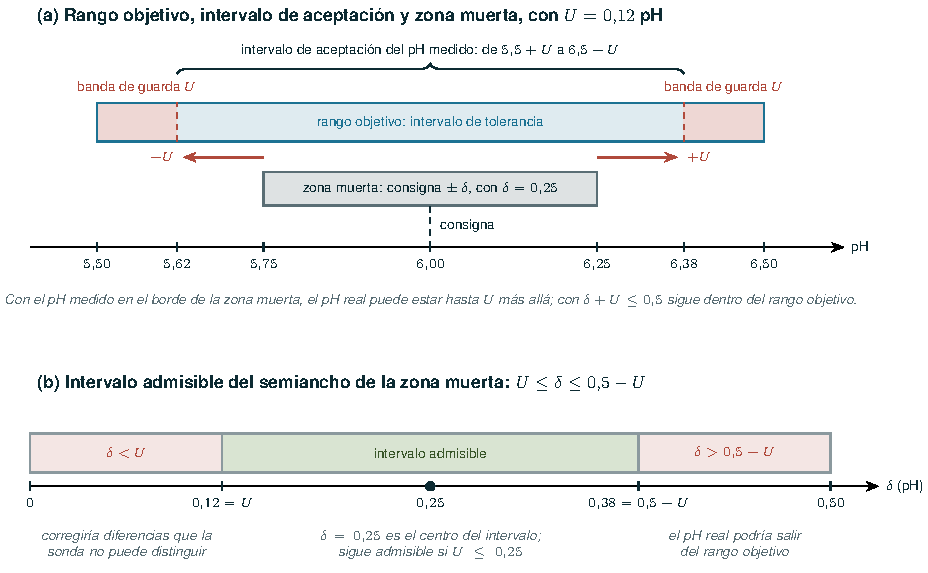
\includegraphics[scale=0.88]{figuras/fig16.pdf}
\caption[Criterio de banda de guarda aplicado a la zona muerta]{Criterio de banda de guarda aplicado a la zona muerta, dibujado a escala con $U=0{,}12$\,pH. (a) Rango objetivo, intervalo de aceptación del pH medido y zona muerta de semiancho $\delta=0{,}25$\,pH: aunque el pH medido quede en el borde de la zona muerta, el real sigue dentro del rango. (b) Intervalo admisible de $\delta$ según la ecuación~\eqref{eq:banda}. Elaborado por los autores (A. Morocho y K. Toledo, TikZ, 2026).}\label{fig:banda}
\end{figure}

La temperatura no se manipula como factor: los ensayos se hacen dentro de una ventana declarada de $22\pm3$\,°C, en la que el error de la compensación es de milésimas de pH (ecuación~\eqref{eq:comp}) y el cambio químico del orden de $\pm0{,}01$\,pH, un orden de magnitud por debajo de $U$. Tampoco se trata como covariable; el intervalo de cada corrida se informa con sus resultados, y el trabajo no puede afirmar el desempeño fuera de la ventana. En cuanto a la concordancia entre resultados, el Vocabulario distingue condiciones de repetibilidad, de precisión intermedia y de reproducibilidad [38]. Con un solo banco no se evalúa la reproducibilidad, sino la repetibilidad dentro de una sesión de calibración y la precisión intermedia entre sesiones; por eso las corridas se reparten en varias sesiones (apartado~\ref{sec:ensayos}).

\subsubsection{Indicadores de dosificación y de productividad}\label{sec:indicadores}
El sistema de dosificación se evalúa con el consumo de ácido y de base y el número de dosis de cada corrida, y con la dosis mínima repetible, su coeficiente de variación y el volumen por revolución al inicio y al final de la campaña, cuya diferencia mide la fatiga del tubo. Estos indicadores miden el desempeño del control, no la productividad del cultivo, que se expresa con el rendimiento por superficie [22], la eficiencia en el uso del agua [30] y el trabajo, del que forma parte la revisión manual del pH [5, 8]. El banco no tiene cultivo, y sus indicadores se relacionan con ellos indirectamente: el tiempo en rango indica cuánto tiempo están disponibles los nutrientes; el consumo se suma a los insumos, y el número de dosis, cuánto interviene el equipo.
